%\documentclass[journal = jpccck, manuscript = article, layout=onecolumn]{achemso}
\documentclass[12pt]{article}
%--------------------   start of the 'preamble'
%
\usepackage{graphicx,amssymb,amstext,amsmath,color}
\usepackage[margin=2cm]{geometry}
\usepackage{abstract}
\usepackage{setspace}
\usepackage[footnotesize,bf]{caption}

% TABLE
\usepackage{multicol,hhline,colortbl,multirow}
\usepackage{braket}
\usepackage{siunitx}
\usepackage{hyperref}
\usepackage{authblk}
\usepackage{siunitx}
\usepackage{mathrsfs}
\usepackage{wrapfig}
%%\usepackage[sort&compress]{natbib}
%%\bibpunct{(}{)}{,}{a}{, }{;}
%
\usepackage[sort&compress]{natbib}
\bibpunct{[}{]}{,}{s}{}{;}


\definecolor{gray}{gray}{0.8}
\def\mobunits{\square\centi\meter\per\volt\per\second}
\def\gcm{\gram\per\cubic\centi\meter}
\def\ccg{\cellcolor{gray}}

\renewcommand{\labelitemii}{$\circ$}
\renewcommand{\bibname}{References}

\renewcommand\Affilfont{\itshape\scriptsize}

\title{Type I: Machine Learning for Structure-Performance Relationships in Organic Semiconducting Devices}
\author[1]{Matthew L. Jones}
\author[2]{Evan D. Miller}
\author[3]{Bryan Stanfill}
\author[4]{Eric Jankowski}
\affil[1]{mattyjones@boisestate.edu, Micron School of Materials Science and Engineering, Boise State University, Boise ID 83725}
\affil[2]{evanmiller326@boisestate.edu, Micron School of Materials Science and Engineering, Boise State University, Boise ID 83725}
\affil[3]{bryan.stanfill@pnnl.gov, Pacific Northwest National Laboratory, Richland WA 99354}
\affil[4]{ericjankowski@boisestate.edu, Micron School of Materials Science and Engineering, Boise State University, Boise ID 83725}

%%\affiliation{Micron School of Materials Science and Engineering, Boise State University, Boise ID 83725}
%%\email{mattyjones@boisestate.edu}
%\author{Evan D. Miller}
%%\affiliation{Micron School of Materials Science and Engineering, Boise State University, Boise ID 83725}
%%\email{evanmiller326@boisestate.edu}
%\author{Bryan Stanfill}
%%\affiliation{Pacific Northwest National Laboratory, Richland WA 99354}
%%\email{bryan.stanfill@pnnl.gov}
%\author{Eric Jankowski}
%%\affiliation{Micron School of Materials Science and Engineering, Boise State University, Boise ID 83725}
%%\email{ericjankowski@boisestate.edu}
\date{}

\begin{document}
\maketitle

%\begin{figure}[h!]\centering
%	\includegraphics[width=0.5\textwidth]{Figures/PublishedHoleMob.pdf}
%    \caption{The mobility trend observed as a function of increasing temperature}
%	\label{fig:MSD}
%\end{figure}

The goal of the proposed work is to understand electron and hole transport in organic semiconductors, combating global climate change through the production of high-efficiency, low cost solar panels. 
The challenge we address here is understanding how the chemistry and packing of photoactive molecules affects the motion of electrons and holes in the organic active layer.
Ordinarily, this requires the execution of a large number of slow quantum chemical calculations to predict the electronic properties of the materials, demanding large amounts of time and computing power.
Our hypothesis is that machine learning techniques, trained on a small subset of quantum chemical data, can be used to predict the electronic capabilities of nanostructure morphologies.
This will dramatically reduce the number of expensive calculations to be performed and facilitate high-throughput parameter-sweep studies of the vast phase space of candidate chemistries and processing methodologies, with the aim of developing a robust set of design-rules for manufacturing efficient devices.


Organic semiconductors are becoming an increasing popular alternative to conventional inorganics in the construction of electronic devices\cite{Tsumura1986,Friend1999,Sariciftci1992} thanks to recent advances in synthetic chemistry and scalability of low-cost manufacturing processes.
However, the efficiency of organic devices (and particularly organic photovoltaics) tends to be significantly lower than conventional devices.
In particular, the charge-carrier mobility describes the speed at which electrons and holes can move through the active layer of the device, and is a crucial descriptor of device efficiency\cite{Sirringhaus2014}.
The mobility depends sensitively on the morphology of the active layer, which describes the relative positions and orientations of the component molecules.
Therefore, in order to manufacture the most efficient devices, it is vital to optimize the morphology such that the charge-carrier mobility is maximized.
The molecular morphology can be influenced by the choices of chemistries in the system, as well as the device processing conditions such as temperature, pressure, solvent choice, and annealing duration\cite{Noriega2013}.
This massive phase space necessitates the use of computational methods (rather than manufacturing hundreds of millions of test devices in a wet lab) that are capable of spanning multiple length- and time-scales.

\clearpage
\begin{wrapfigure}{lb}{0.5\textwidth}\centering
%\begin{figure}[h!]\centering
%\vspace{1em}
	\includegraphics[width=0.5\textwidth]{Figures/fig.png}
    %\begin{tabular}{cc}
    %    \includegraphics[width=0.5\textwidth]{Figures/morphologySpam.png} &
	%    \includegraphics[width=0.5\textwidth]{Figures/flowchartFull.png}
    %\end{tabular}
    \caption{Predicting charge mobility for a single simulation snapshot requires quantum chemical calculations be performed on each pair of chromophores. Machine learning techniques represent a way to obtain electronic transfer integrals between chromophore pairs, saving potentially billions of unnecessary, expensive chemical calculations per semiconductor study.}
	\label{fig:fig1}
%\end{figure}
\end{wrapfigure}

Carriers move through the morphology via quantised tunnelling events - `hops' - between electronically active functional groups on the molecules known as `chromophores'.
The rate at which a carrier hop can occur from chromophore $i$ to chromophore $j$, $k_{ij}$, is given by the semi-classical Marcus expression\cite{Marcus1964}:
\begin{equation}\label{eq:Marcus}
    k_{ij} = \frac{\left| T_{ij} \right|^{2}}{\hbar} \sqrt{\frac{\pi}{\lambda k_{B} T}} \exp \left[ - \frac{(\Delta E_{ij} + \lambda)^{2}}{4 \lambda k_{B} T} \right],
\end{equation}
where $T_{ij}$ is the electronic transfer integral, $\Delta E_{ij}$ is the difference in energy between the initial and final hop sites, and the remaining parameters are material-specific, thermodynamic or fundamental constants.
The speed at which a hop from one chromophore to a neighbour can occur is primarily governed by $T_{ij}$, which is a measure of the amount of molecular orbital overlap between the pair.
%A large transfer integral describes an easy hop, which can happen quickly, leading to a fast charge carrier, a high carrier mobility, and a more efficient device.

Current state-of-the-art predictions of mobility combine computational techniques: molecular dynamics simulations to obtain a candidate morphology, quantum chemical calculations to determine the transfer integrals and hop rates between chromophores, and kinetic Monte Carlo to simulate charge motion through the device (Figure \ref{fig:fig1})\cite{MorphCT,Jones2016,Jones2017}.
These simulations can take several days to run on supercomputers even with GPU acceleration hardware for just a single selection of component molecules and device processing techniques.
Optimizing the simulation pipeline will dramatically improve computational throughput of the screening process required to detect combinations of molecules and processing that will result in the most efficient devices.
One area of opportunity we have identified is the calculation of transfer integrals via quantum chemical calculations: of the 1,000-100,000 chromophore pairs that make up a single simulation snapshot.
Many pairs share the same local structure and therefore have the same transfer integrals.
Performing quantum chemical calculations for each pair of chromophores therefore represents an inefficiency compared to a sufficiently accurate pattern recognition scheme that can look up transfer integrals based on their local structure.

We propose using machine learning techniques to streamline the quantum chemical portion of the pipeline by predicting carrier transfer integrals between pairs of chromophores.
Our preliminary work has investigated a semi-crystalline test system containing 1,000 oligomers of poly(3-hexylthiophene), each of length 15 monomers.
For each pair of nearest-neighbour monomers, we use semi-empirical quantum chemical calculations to predict the electronic transfer integrals, for a total of 40,000 data points.
In general, monomers are defined by the locations of their constituent atoms and bonds, and the transfer integral can be determined by considering the relative position of each monomer to its neighbour.
As such, we consider only geometric descriptors for each pair, constructed from 6 independent labels corresponding to relative translations in three dimensions, and relative rotations around three orthogonal axes.

At MATDAT18, we explored the efficacy of linear models (e.g, simple linear regression and semi-parametric penalized splines) as well as artificial neural networks and kernel-based methods (e.g., support vector machines) in predicting the transfer integrals, each of which were trained using a selection of the 40,000 data points.
The spline based approaches were able to identify meaningful change points within each feature as well as the interactions between features, however, the strict linear form of these models proved too restrictive to adequately predict the non-linear relationship between the features and the transfer integral.
This non-linear relationship was replicated well by the neural networks (deep and shallow), which were able to predict the transfer integral with reasonable accuracy, but they lack transparent feature importance metrics that would afford us a deeper knowledge of how these features interact in nature.
Random-forest decision tree techniques proved to be both the most accurate and produced transparent feature importance metrics.
The random forest fits resulted in a correlation coefficient of $r^{2} = 0.978$, corresponding to an average absolute error of 30 meV, far below the expected 100 meV accuracy of even the most computationally intensive quantum chemical predictions.
%\textcolor{red}{$<$I expect Bryan will have more to say about this section$>$}


%\subsection{Why is a continuation warranted and promising?}

The small average errors in our predictions provide an extremely promising `proof-of-concept' for machine learning techniques to be able to evaluate tens of thousands of transfer integrals \textit{in situ} in a matter of minutes instead of days.
\begin{wrapfigure}{lb}{0.5\textwidth}\centering
	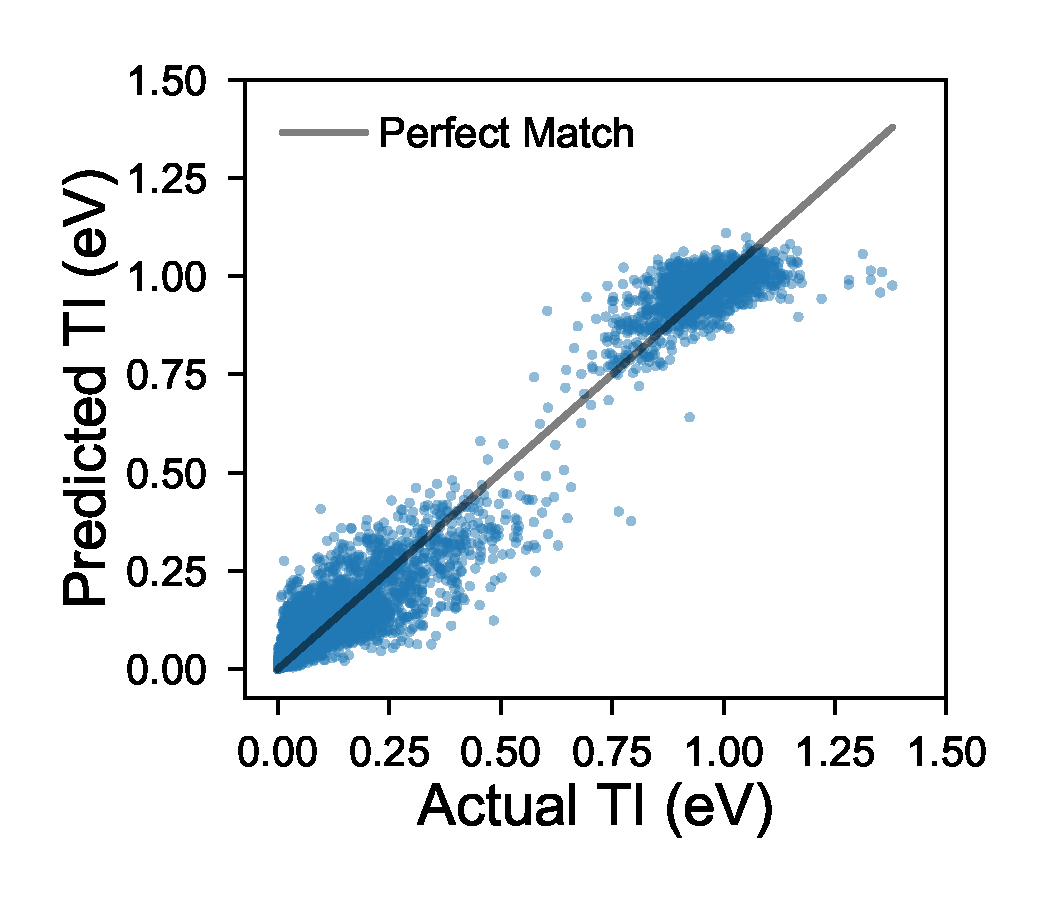
\includegraphics[width=0.5\textwidth]{Figures/comparison.pdf}
    \caption{
The comparison of the transfer integrals for an ordered donor polymer system calculated by ZINDO/S compared to those predicted by the random forest.
This produces an average absolute error of 30 meV and an $R^2$ value of 0.978.
}
	\label{fig:random_forest_results}
%\end{figure}
\end{wrapfigure}
Figure \ref{fig:random_forest_results} shows that there is still room for further optimization of our model to provide more accurate predictions of the TI.
We intend to determine which descriptors (or combinations thereof) are required in order to tighten up the model and reduce the average error still further, to a target value of 10 meV.
The transferability of this model to other statepoints and chemistries also needs to be thoroughly investigated.
For instance, how does the accuracy of the model change for replicant systems processed at the same statepoint?
If we now consider the same molecules but processed at a different statepoint, resulting in a different nanostructure, do we need to re-calibrate our model in order to obtain the same high level of accuracy?
What about if we consider a different polymer, or a different chemistry entirely (for instance, a small molecule system, or blends of multiple molecule types)?


%\subsection{Why is this important to materials research?}
Ideally, we will be able to configure our model to be as chemistry and processing agnostic as possible to allow maximum transferability to other organic systems.
This will allow the wider materials science community to predict electronic properties for a wide database of molecules that we expect to release to the research community through open-source hosting methods.
A sufficiently accurate model can be used instead of quantum chemical calculations, resulting in a marked decrease in computation time and resources required by organic researchers, and faster identification of candidate chemistries and processes.
Open data repositories such as the Harvard Clean Energy Project database contain millions of candidate molecules - a currently untenably large dataset for investigating charge transport properties using quantum chemical techniques.
Our work here will allow researchers to investigate many more of these molecules at many more statepoints in the same amount of time, helping us to more strongly connect morphology and performance, leading us closer to a set of design rules for the most efficient devices.


\subsection{What could be achieved with additional resources?}


Our current database of quantum chemical calculations consists of around 500 unique morphologies, covering 10 chemistries including polymers, fullerenes, block co-polymers and polycyclic aromatic hydrocarbons, each with at least 3 processing state points above and 3 state points below an order-disorder transition temperature for each chemistry.
This corresponds to the electronic properties data for over 10,000,000 chromophore pairs, although a portion of these ($\sim$20\%) are unnecessary `repeat' calculations resulting in negligible transfer integrals.
With additional resources, we can increase the accuracy of our current models, and determine their transferrability to other statepoints and chemistries.
According to our preliminary results, calibrating a model for a single statepoint appears to have good transferability to other statepoints, suggesting that in the worst-case scenario is that we require the generation of a new model for each new chemistry, which can then be used to predict a wide range of statepoints.
% Probably want to include one or both of the graphs Evan made on Tuesday night here to prove our claim?
Even in this case, performing a set of quantum chemical calculations for the top 50 most promising candidates according to the Clean Energy Project database seems reasonable.
The improved runtime of the machine learning models will then permit us to expand our transfer integral database to include dramatically more statepoints for each system - aiming for 20 to 30 statepoints per chemistry, in order to fully explore the morphology landscape of the molecular blend.
We then intend to make our transfer integral database freely available to the research community to assist further exploration of organic semiconductor behaviour.


\subsection{Why is this important to data science?}


A data science shortcoming exposed by this material problem is the fact that so many modern analytical techniques are geared towards the big data problem both in the feature space and dataset size.
In this problem, there are a large number of data points to train on, but the feature set is relatively small ($\approx$10 features).
Compounding this issue is the highly non-linear relationship between the features and output, which makes it difficult to faithfully model with most machine learning techniques.
Over the course of MATDAT18, we used data visualizations and measures of correlation to define feature interactions that were then fed into various machine learning algorithms.
However, very few of them proved to play a role in the final model.
Data driven interactions identified by the semi-parametric spline regressions and random forests proved much more predictive, but we believe more, higher-order interactions that have not yet been identified could further improve the model.
To accomplish this, more sophisticated variable search algorithms, e.g.~genetic algorithms, will need to be modified for this purpose.
Specifically, we propose to use feature engineering to drastically expand our feature space then genetic algorithms to identify those that are the most predictive of transfer integral.


\subsection{Budget}

$<$ Eric's doing this bit $>$


\subsection{External data resources and cyberinfrastructure}

All preliminary data has been generated using the open source MorphCT\cite{Jones2017}, HOOMD-Blue\cite{Anderson08}, and ORCA\cite{Neese2012b} software suites, and are currently hosted online by the Albertson's Library at Boise State University\cite{MatDat18Data}.
The morphologies were generated using local computing hybrid CPU/GPU infrastructure at Boise State University, supported by the National Science Foundation under Grant No 1229709.
This work also used the Extreme Science and Engineering Discovery Environment (XSEDE), which is supported by National Science Foundation Grant Number ACI-1053575.
These resources will be also be available for subsequent data generation for this proposal.
In addition, we have access to a further 5,000 SUs through XSEDE on the high-performance GPU cluster XSTREAM, with the intent to apply for an increase to that allocation in the future.

\newpage


\bibliography{refs}
\bibliographystyle{unsrt}

\end{document}
